%&pdflatex

\documentclass[12pt]{article}

\usepackage[spanish, es-tabla]{babel}
\usepackage{enumerate}
\usepackage{lscape}
\usepackage{vmargin}
\usepackage{pdfpages}
\usepackage{fancyhdr}
\usepackage{graphicx}
\usepackage{float}
\usepackage{titlesec}
\usepackage[bottom]{footmisc}
\usepackage[hidelinks]{hyperref}
\usepackage{listings}
\usepackage{color}
\usepackage{colortbl}
\usepackage{xcolor}
\usepackage{amsmath}
\usepackage{array}
\usepackage{svg}
\usepackage{pgfgantt}
\usepackage[T1]{fontenc}
\usepackage[sfdefault]{AlegreyaSans} %% Option 'black' gives heavier bold face
%% The 'sfdefault' option to make the base font sans serif
\renewcommand*\oldstylenums[1]{{\AlegreyaSansOsF #1}}


%*******************************************************************************
\extrarowheight = -0.3ex
\renewcommand{\arraystretch}{2.25}
\setpapersize{A4}
\hypersetup{
    colorlinks=true,
    linkcolor=blue,
    urlcolor=purple,
    citecolor=black, 
    linktocpage=true,
}
\definecolor{gray95}{gray}{.95}
\definecolor{gray75}{gray}{.75}
\definecolor{barblue}{RGB}{153,204,254}
\definecolor{groupblue}{RGB}{51,102,254}
\definecolor{linkred}{RGB}{165,0,33}
\lstset{
    frame=Ltb,
    framerule=0pt,
     aboveskip=0.5cm,
     framextopmargin=3pt,
     framexbottommargin=3pt,
     framexleftmargin=0.4cm,
     framesep=0pt,
     rulesep=.4pt,
     backgroundcolor=\color{gray95},
     rulesepcolor=\color{cyan},
     %
     stringstyle=\ttfamily,
     showstringspaces = false,
     basicstyle=\small\ttfamily,
     commentstyle=\color{cyan},
     keywordstyle=\bfseries\color{purple},
     %
     numbers=left,
     numbersep=15pt,
     numberstyle=\small,
     numberfirstline = false,
     breaklines=true,
}

%minimizar fragmentado de listados
\lstnewenvironment{listing}[1][]
   {\lstset{#1}\pagebreak[0]}{\pagebreak[0]}


\lstdefinestyle{C}
   {
       language=C++,
   }

\lstdefinestyle{python}
    {
        language=Python,
    }

\setcounter{secnumdepth}{4}
%*******************************************************************************
%   Adding a new level of section --> subsubsubsection
%******************************************************************************
\titleclass{\subsubsubsection}{straight}[\subsection]

\newcounter{subsubsubsection}[subsubsection]
\renewcommand\thesubsubsubsection{\thesubsubsection.\arabic{subsubsubsection}}
\renewcommand\theparagraph{\thesubsubsubsection.\arabic{paragraph}} % optional; useful if paragraphs are to be numbered

\titleformat{\subsubsubsection}
  {\normalfont\normalsize\bfseries}{\thesubsubsubsection}{1em}{}
\titlespacing*{\subsubsubsection}
{0pt}{3.25ex plus 1ex minus .2ex}{1.5ex plus .2ex}

\makeatletter
\renewcommand\paragraph{\@startsection{paragraph}{5}{\z@}%
  {3.25ex \@plus1ex \@minus.2ex}%
  {-1em}%
  {\normalfont\normalsize\bfseries}}
\renewcommand\subparagraph{\@startsection{subparagraph}{6}{\parindent}%
  {3.25ex \@plus1ex \@minus .2ex}%
  {-1em}%
  {\normalfont\normalsize\bfseries}}
\def\toclevel@subsubsubsection{4}
\def\toclevel@paragraph{5}
\def\toclevel@paragraph{6}
\def\l@subsubsubsection{\@dottedtocline{4}{7em}{4em}}
\def\l@paragraph{\@dottedtocline{5}{10em}{5em}}
\def\l@subparagraph{\@dottedtocline{6}{14em}{6em}}
\makeatother

\setcounter{secnumdepth}{4}
\setcounter{tocdepth}{4}

%*****************************************************************************

\begin{document}

  \begin{titlepage}
    \centering
   {\bfseries\Large Universidad Carlos III de Madrid \par}
    \vspace{5cm}
    {\scshape\Huge Informe del Trabajo de Evaluación del Bloque 1 \par}
    \vspace{2cm}
    {\itshape\Large Diseño de circuitos electrónicos para comunicaciones}
    \vfill
    {\Large Autores: \par}
    \vspace{1cm}
    {\Large Markel Serrano y Daniel Theran}
    \vfill
    {\Large 11 de Octubre del 2022 \par}
  \end{titlepage}

  \section*{Apartado 1}

    \paragraph*{}
    En este apartado se pedía diseñar un filtro paso bajo en \textbf{Matlab} de forma que contase con un polo en la frecuencia de 30KHz.
    Para ello, es necesario utilizar la función "tf", que calcula la función de transferencia en tiempo continuo (H(s)).
    Después, transformamos esta función en H(z) mediante el uso del comando "c2d", que nos calcula la transformada Z de la función anterior.
    De esta forma, el código para generar las anteriores funciones, así como las variables necesarias y su correspondiente salida:

    \begin{figure}[H]
      \centering
      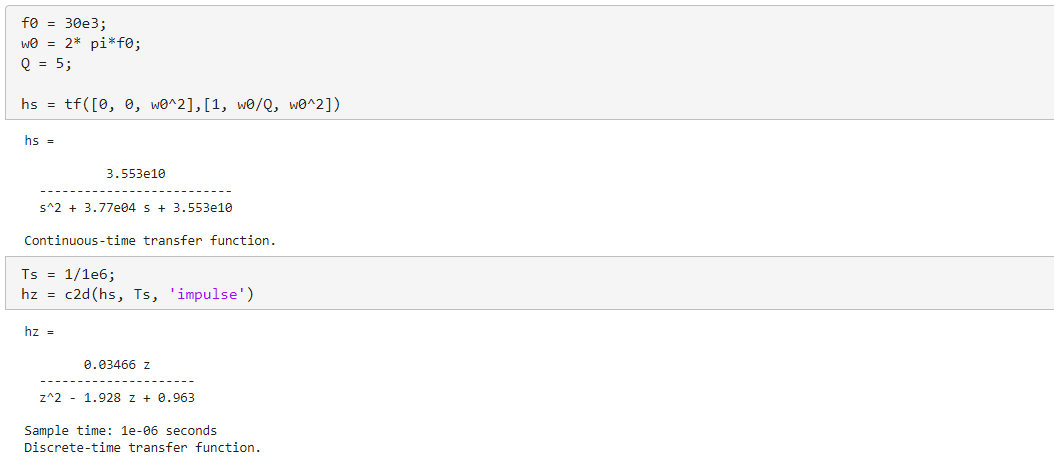
\includegraphics[width=1\linewidth]{Img/img_apartado_1.PNG}
      \caption{Entrada y salida del apartado 1 en Matlab}%
      \label{fig:img1}
    \end{figure}

    %%si quieres, tras esto se puede explicar un poco el significado de la función Hz, aunque tampoco le veo mucho sentido. Igual es mejor explicarlo en el apartado siguiente

  \section*{Apartado 2}
  
    \paragraph*{}
    En el segundo apartado se pide representar gráficamente ambas funciones. Para conseguir este objetivo se emplea la función "bode".
    De esta forma, la representación de la función de transferencia, tanto en tiempo continuo como en discreto, queda de la siguiente manera:

    \begin{figure}[H]
      \centering
      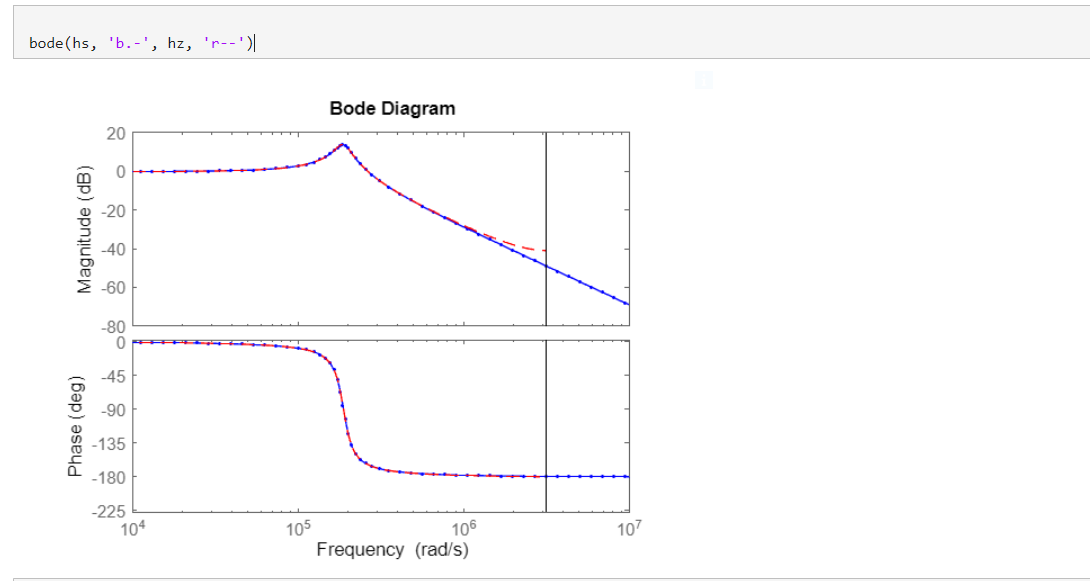
\includegraphics[width=1\linewidth]{Img/img_apartado_2.PNG}
      \caption{H(s) y H(z) representados en Matlab}%
      \label{fig:img2}
    \end{figure}

    \paragraph*{}
    Como se puede ver,

    %%falta tirarnos el moco con alguna explicación técnica
  
  \section*{Apartado 3}

  \paragraph*{}
    En esta sección se analiza tanto analíticamente como gráficamente, a través del software de simulación de circuitos \textbf{LTSpice}, 
    una de las etapas del circuito completo dado en el ejercicio. 
    
    \paragraph*{}
    El fichero de simulación que se nos facilita corresponde a una de las etapas del circuito completo. 
    Concretamente sería la etapa cuya salida corresponde a un filtro paso bajo (\textit{Vlp}). Sin embargo, 
    cuando se analiza por separado dicha etapa, se puede observar que tanto su función de transferencia como 
    su análisis en \textbf{LTSpice}, corresponden con un filtro paso bajo. 

    \paragraph*{}
    La función de transferencia de ésta primera etapa del filtro, a la que se ha llamado $H_{1}(Z)$, es la siguiente: 
    
    \begin{figure}[H]
        \begin{center}
            $H_{1}(Z) = \frac{C_{1}}{C_{2} + C_{7}}\cdot\frac{Z^{-1}}{1 - \frac{C_{2}}{C_{2} + C_{7}}\cdot Z^{-1}}$
            \caption{Función de transferencia de la primera etapa del circuito completo}%
            \label{fig:h1}
        \end{center}
    \end{figure}
    
    \paragraph*{}
    Como se puede observar, da como resultante un filtro no inversor y con retardo, el cual nos afectará más adelante en la función de transferencia 
    del circuito completo. El desarrollo de función de transferencia (\ref{fig:h1}), se encuentra disponible en el Anexo I.


  \section*{Apartado 4}
  \section*{Apartado 5}
    \paragraph*{}
    En esta sección se va a analizar de forma analítica la función de transferencia del circuito completo. Para ello primero tenemos que 
    identificar qué otras etapas existen en el mismo y sacar sus correspondientes funciones de transferencia, de forma que finalmente, 
    podamos analizar por bloques el funcionamiento completo del circuito y sacar la función de transferencia del mismo. 

    \begin{figure}[H]
        \centering
        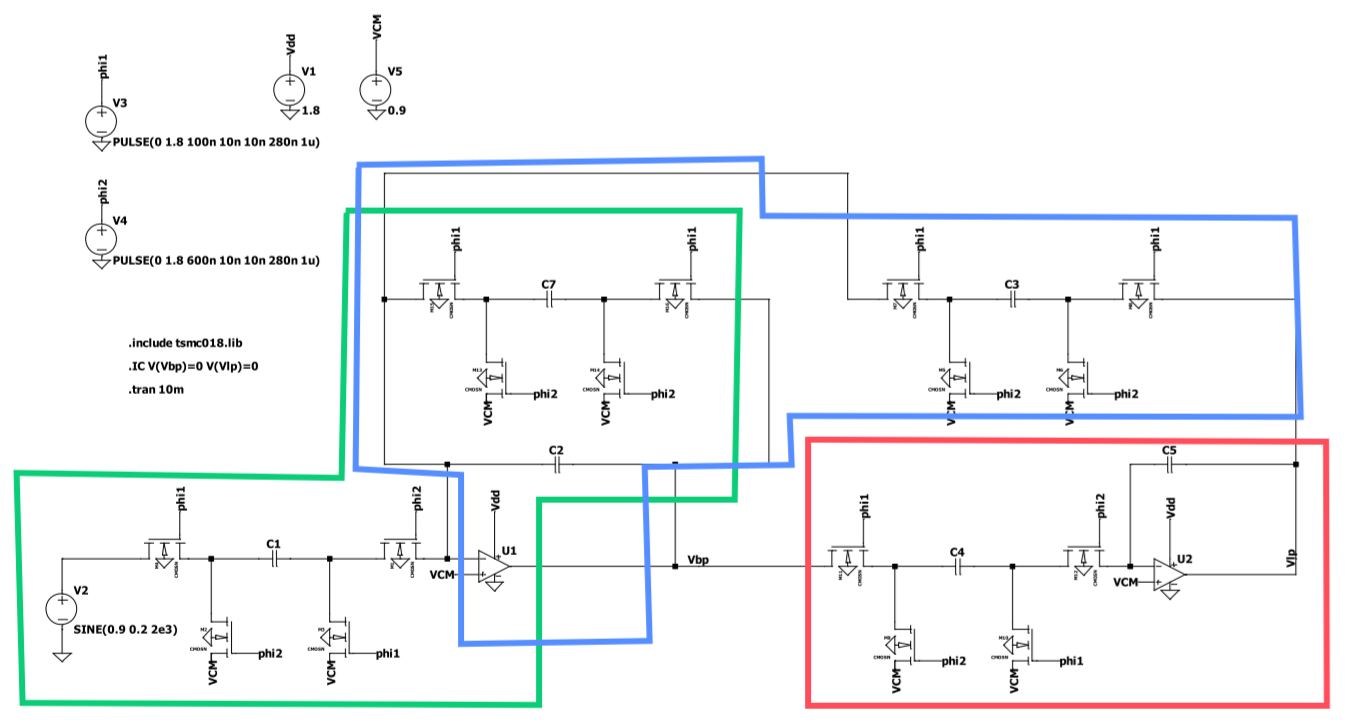
\includegraphics[width=1\linewidth]{Img/Etapas_Filtro.png}
        \caption{Etapas del circuito completo}%
        \label{fig:etapas}
    \end{figure}
    
    \paragraph*{}
    En la figura \ref{fig:etapas} podemos diferenciar 3 etapas:

    \begin{itemize}
        \item \textbf{Integrador:} Enmarcada en rojo, es la correspondiente con la fase integradora del circuito 
        \item \textbf{Filtro 1 ($H_1$):} Enmarcada en azul, es el correspondiente con la primera fase del filtro, el cual se ha analizado en el apartado 3. 
        \item \textbf{Filtro 2 ($H_2$):} Enmarcada en verde, es otra etapa del circuito que, como veremos más adelante, corresponde con un filtro inversor sin retardo.
    \end{itemize}
    
    \subsection*{Función de transferencia de la etapa 2.}

    \paragraph*{}
    La función de transferencia de la etapa 2, a la que se ha llamado $H_{2}(Z)$, es la siguiente: 

    \begin{figure}[H]
        \begin{center}
            $H_{2}(Z) = - \frac{C_{3}}{C_{2} + C_{7}}\cdot\frac{1}{1 - \frac{C_{2}}{C_{2} + C_{7}}\cdot Z^{-1}}$
            \caption{Función de transferencia de la segunda etapa del circuito completo}%
            \label{fig:h2}
        \end{center}
    \end{figure}

    \paragraph*{}
    Como se puede observar, da como resultante un filtro inversor y sin retardo. Esto hará posible que el funcionamiento del circuito completo tenga sentido 
    y sea realizable. El desarrollo de función de transferencia (\ref{fig:h2}), se encuentra disponible en el Anexo I.

    \subsection*{Función de transferencia de la etapa 3 o etapa integradora.}

    \paragraph*{}
    La función de transferencia de la etapa 3, a la que se ha llamado $H_{3}(Z)$, es la siguiente:
    
    \begin{figure}[H]
        \begin{center}
            $H_{3}(Z) = \frac{C_{4}}{C_{5}}\cdot\frac{Z^{-1}}{1 - Z^{-1}}$
            \caption{Función de transferencia de la tercera etapa del circuito completo}%
            \label{fig:h3}
        \end{center}
    \end{figure}

    \paragraph*{}
    Se puede ver que se trata de un integrador ya que tiene un polo en 0 Hz (resolviendo el denominador) y aplica un retardo a la salida. Dicho retardo lo vamos a ver 
    en la función de transferencia del circuito completo. El desarrollo de la función de transferencia de esta etapa (\ref{fig:h3}), se encuentra disponible en el Anexo I. 

    \paragraph*{}
    Una vez calculada las funciones de transferencia de las 3 etapas que se pueden diferenciar en el circuito, debemos ver como es el funcionamiento completo del circuito 
    mediante un diagrama de bloques. 

    \begin{figure}[H]
        \centering
        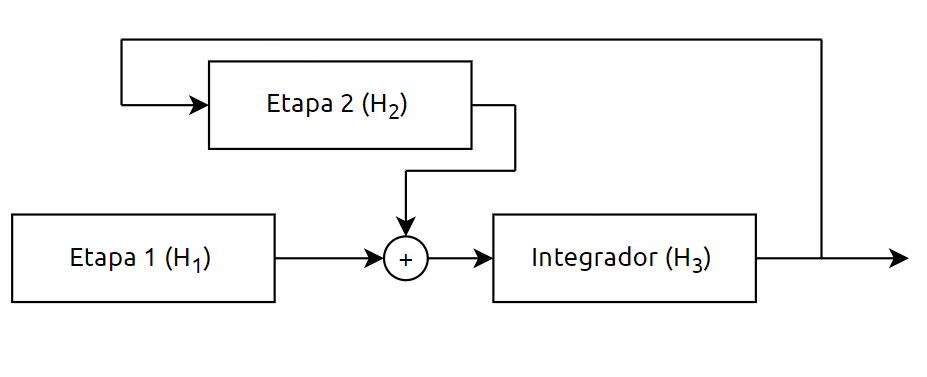
\includegraphics[width=1\linewidth]{Img/Blouques_circuito.png}
        \caption{Bloques de funcionamiento del circuito}%
        \label{fig:bloques}
    \end{figure}
    
    \paragraph*{}
    Si analizamos el funcionamiento interno entre estos bloques y vemos como interactúan las señales de entrada y salida de cada bloque, 
    observamos que la función de transferencia completa del circuito es de la forma:

    \begin{figure}[H]
        \begin{center}
            $H(Z) = \frac{H_{1}\cdot H_{3}}{1 - H_{2}\cdot H_{3}}$
            \caption{Función de transferencia del circuito completo en bloques}%
            \label{fig:h_prev}
        \end{center}
    \end{figure}

    \paragraph*{}
    Sustituyendo en los valores de $H_{1}$, $H_{2}$ y $H_{3}$ en \ref{fig:h_prev} y simplificando, obtenemos la siguiente función de transferencia: 

    \begin{figure}[H]
        \begin{center}
            $H(Z) = \frac{C_{1}C_{4}\cdot Z^{-2}}{C_{2}C_{5}\cdot Z^{-2} + (C_{4}C_{3} - C_{5}C_{7} - 2C_{5}C_{2})\cdot Z^{-1} + C_{5}(C_{2} + C_{7})}$
            \caption{Función de transferencia del circuito completo en Z inversa}%
            \label{fig:h_inv}
        \end{center}
    \end{figure}

    \paragraph*{}
    Si resolvemos para tener términos en Z y no en Z inversa: 

    \begin{figure}[H]
        \begin{center}
            $H(Z) = \frac{C_{1}C_{4}}{C_{5}(C_{2} + C_{7})\cdot Z^{2} + (C_{4}C_{3} - C_{5}C_{7} - 2C_{5}C_{2})\cdot Z + C_{2}C_{5}}$
            \caption{Función de transferencia del circuito completo}%
            \label{fig:h_z}
        \end{center}
    \end{figure}

    \paragraph*{}
    Donde los términos cuadráticos del denominador los llamamos \textbf{A}, los lineales \textbf{B} y el término independiente \textbf{C}. Ésto nos sirve 
    para posterior mente fijar los valores de los condensadores de manera que obtengamos un filtro paso bajo con un comportamiento similar al filtro del 
    apartado 1, es decir, con un polo de funcionamiento en 30 kHz. 

    \paragraph*{}
    La función de transferencia final queda entonces de la forma: 

    \begin{figure}[H]
        \begin{center}
            $H(Z) = \frac{a_{0}}{A\cdot Z^{2} + B\cdot Z + C}$
            \caption{Función de transferencia del circuito completo simplificada}%
            \label{fig:h}
        \end{center}
    \end{figure}

    \paragraph*{}
    Siendo las relaciones entre los coeficientes de la función y los condensadores, la siguiente: 
    
    \begin{itemize}
        \item $a_{0} \rightarrow C_{1}C_{4}$
        \item $A \rightarrow C_{5}(C_{2} + C_{7})$
        \item $B \rightarrow (C_{4}C_{3} - C_{5}C_{7} - 2C_{5}C_{2})$
        \item $C \rightarrow C_{2}C_{5}$
    \end{itemize}

    \paragraph*{}
    En el apartado 7 veremos que para poder comparar los valores A, B y C de la función de transferencia total con el filtro obtenido en el 
    apartado 1 (filtro de matlab), hay que normalizar los elementos de la función al término cuadrático del denominador. 

  \section*{Apartado 6}
  \section*{Apartado 7}

    \paragraph*{}
    Para calcular valores de los condensadores tales que hagan al circuito diseñado comportarse como el circuito teórico del primer apartado,
    sus funciones de transferencia deben ser equivalentes. Para ello, se iguala término a término la función de transferencia teórica obtenida en el primer apartado
    con la función de transferencia calculada en el apartado 5, una vez se ha normalizado el término cuadrático de ambas funciones. Además, debemos suponer que los valores de C2 y C5 son iguales, e iguales a 20pF,
    y C1 y C4 son a su vez iguales.

    %%me parecía redundante meter aquí la expresión completa de las funciones cuando ya están en el apartado 1 y 5
    \paragraph*{}
    De esta forma, encontramos las siguientes equivalencias:
    
    \begin{itemize}
      \item $\frac{C_2}{C_2 + C_7} = 0.963$ 
      \item $\frac{C_1 \cdot C_4 }{C_5(C_2+C_7)} = 0.03466$
      \item $\frac{C_4\cdot C_3 - C_5 \cdot C_7 - 2 \cdot C_5 \cdot C_2}{C_5(C_2 + C_7)} = -1.928$
    \end{itemize}

    \paragraph*{}
    Despejando de las anteriores equivalencias, se obtienen los siguientes valores para los condensadores del circuito:

    \begin{itemize}
      \item $C_2 = C_5 = 20pF$
      \item $C_1 = C_4 = 3.79pF$
      \item $C_7 = 0.77 pF$
      \item $C_3 = 3.82pF$
    \end{itemize}


 \section*{Apartado 8}
 \section*{Apartado 9}
 \paragraph*{}
 En este apartado se pide calcular todas las resistencias equivalentes de las redes de capacidad conmutada. Para realizar este cambio,
 se pueden sustituir los condensadores $C_1, C_7, C_3$ y $C_4$, así como sus transistores correspondientes, por la resistencia equivalente en
 cada caso.

 \paragraph*{}
 Para calcular el valor de la resistencia equivalente, hay que dividir el voltaje medio medido en cada condensador por la corriente media
 que atraviesa dicho elemento. No obstante, de manera analítica puede calcularse como $\frac{T_s}{C}$. Así, las resistencias equivalnetes son las siguientes:

 \begin{itemize}
  \item $R_1 = R_4 = 263.85K\Omega $
  \item $R_7 = 1.3 M\Omega$
  \item $C_3 = 261.78K\Omega$
\end{itemize}
 \newpage
 \section*{Anexos: }
 \subsection*{Anexo I: Desarrollo de la función de transferencia de la primera etapa del filtro completo}
 \subsection*{Anexo II: Desarrollo de la función de transferencia del filtro completo}
\end{document}
